\documentclass[sans,aspectratio=169]{beamer}
\usepackage[utf8]{inputenc}
\usepackage[english,russian]{babel}
\usepackage{graphicx}
\usepackage{tikz}
\usepackage[inkscapelatex=false]{svg}
\usepackage{setspace}
\usepackage{listings} % код с++

\usepackage{amsmath}
\usepackage{mathtools} 
\usepackage{bm}

\usepackage{fixltx2e}

\usepackage{tabularray}
\usepackage[hmargin=1cm]{geometry}

% to fix contrast on includegraphics slides in adobe
\usepackage{eso-pic}
\AddToShipoutPicture{%
\makeatletter%
\special{pdf: put @thispage <</Group << /S /Transparency /I true /CS /DeviceRGB>> >>}%
\makeatother%
}

\DeclareRobustCommand{\frac}[3][0pt]{%
	{\begingroup\hspace{#1}#2\hspace{#1}\endgroup\over\hspace{#1}#3\hspace{#1}}}



\usepackage[sfdefault]{noto-sans}
\usepackage[T1]{fontenc}

% Тема и цвет шапки у слайда
\definecolor{myblue}{RGB}{51, 51, 178}
\usetheme{Boadilla}
\usecolortheme{seahorse}
\setbeamercolor{frametitle}{fg=white,bg=myblue}

% Низ слайда
\setbeamertemplate{navigation symbols}{}
\setbeamertemplate{footline}[page number]
\setbeamercolor{footnote}{fg=myblue, bg=myblue}

% Инфа pdf
\title[Государственный университет «Дубна»]{Презентация ВКР}
\author[Д.А. Никулин]{Д.А. Никулин, nda.19@uni-dubna.ru}
\institute[САУ]{Институт системного анализа и управления}
\date[08.06.2023]{}

%\graphicspath{{pic/}}
\usefonttheme[onlymath]{serif}
\setbeamertemplate{frametitle}[default][left]


% Уменьшить лейблы itemize и enumerate
\setbeamertemplate{itemize item}{\scriptsize\raise1.5pt\hbox{\donotcoloroutermaths$\blacktriangleright$}}

\begin{document}
%********************************TITLE********************************************%

% 1
\begin{frame}[noframenumbering,plain]
	

	\vskip10mm
	
	\definecolor{myblue}{RGB}{51, 51, 178}
	\setbeamercolor{block body example}{bg=myblue}
	\begin{exampleblock}{}
		{
			\vskip3mm
			\begin{center}
				
				\begin{spacing}{1.25}
					\textcolor{white}{\fontsize{15}{16}\selectfont Разработка и оптимизация оценочной функции \\ для учета межмолекулярных взаимодействий \\ в белковых комплексах}
				\end{spacing}
				
			\end{center}
			\vspace{-6mm}
		}
	\end{exampleblock}
	
	\vskip7mm
	
	\centering
	{\fontsize{11}{12}\selectfont {Даниил Никулин}}
	
	\vskip4mm
	\centering
	\fontsize{9}{11}\selectfont
	Государственный университет <<Дубна>>
		
	\vskip1mm
	\fontsize{9}{11}\selectfont Институт системного анализа и управления
	
	\vskip1mm
	\fontsize{9}{11}\selectfont Кафедра распределенных информационно-вычислительных систем


\end{frame}



% 2
\begin{frame}{Постановка задачи}
	\fontsize{11}{15}\selectfont
	\hangindent=-0.5cm
	\hangafter=-1 \noindent
	\setlength{\leftmargini}{20pt}
	


\begin{columns}[c]
	\column{.5\textwidth}
	
	\vspace{4pt}
	
	Кинетический Монте-Карло
	\begin{itemize}
	\setbeamercolor{itemize item}{fg=myblue!60}
	\setlength\itemsep{1mm}
	\item белок-белок взаимодействия
	\item белки как <<твердые>> тела
	\item поступательные и вращательные \\ движения
	\item оценка энергии связывания
	\end{itemize}

	\column{.5\textwidth}
	\vspace{-2pt}
	\begin{center}
		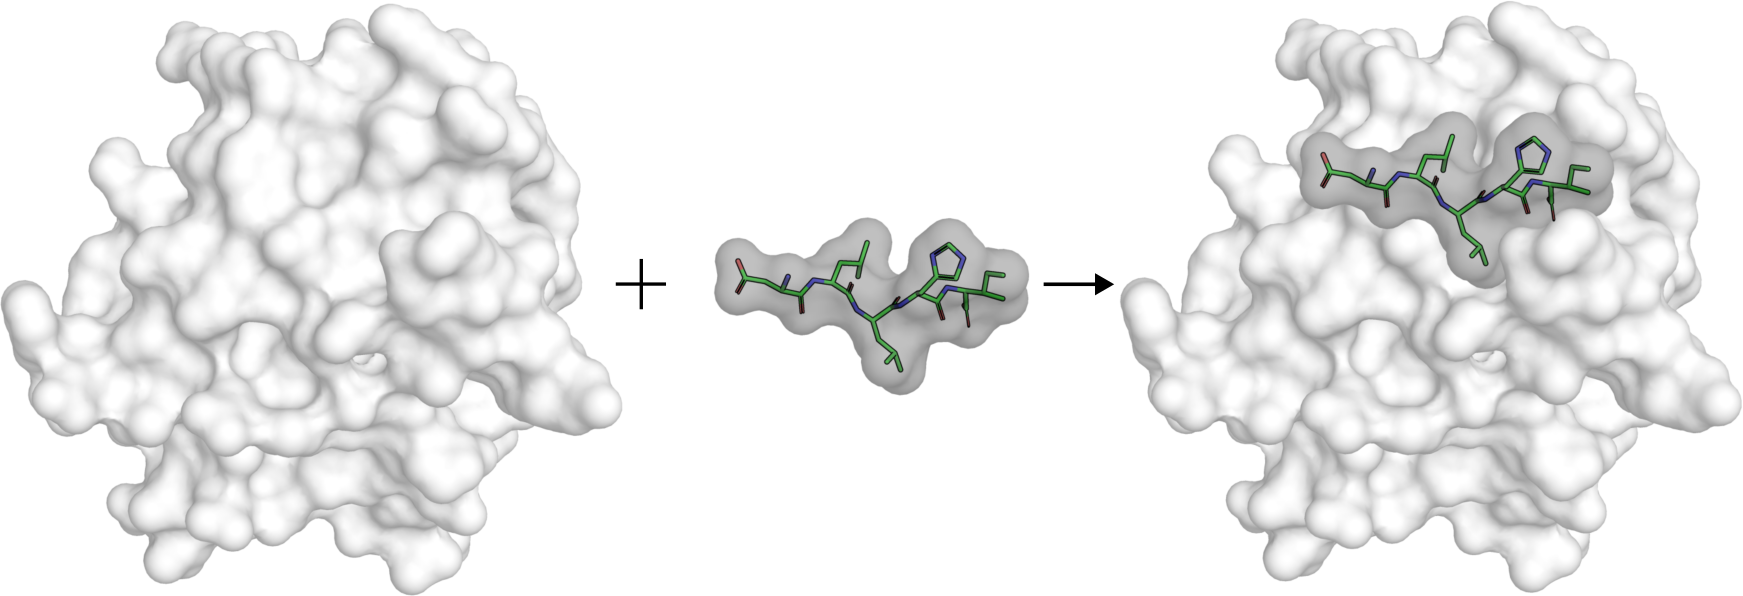
\includegraphics[width=1.0\textwidth]{images/plc.png}
	\end{center}
\end{columns}

\vspace{5pt}

\begin{columns}[c]
	\column{.5\textwidth}
	
	\vspace{-4pt}
		
	Проблемы применения инструментов
	\begin{itemize}
		\setbeamercolor{itemize item}{fg=myblue!60}
		\setlength\itemsep{1mm}
		\item ориентированность на \\ молекулярную динамику
		\item вычислительная сложность 
	\end{itemize}
	
	
	\column{.5\textwidth}
	
	\vspace{18pt}
	
	Оценочная функция
	\begin{itemize}
		\setbeamercolor{itemize item}{fg=myblue!60}
		\setlength\itemsep{1mm} 
		\item нековалентные взаимодействия
		\item силовое поле CHARMM
		\item неявный растворитель EEF1
		\item $F_{score} = E_{vdw} + E_{coulomb} + E_{solvent}$
	\end{itemize}

\end{columns}

\end{frame}



% 3
\begin{frame}{Потенциал Леннарда-Джонса}
	\fontsize{11}{15}\selectfont
	\hangindent=-0.5cm
	\hangafter=-1 \noindent
	\setlength{\leftmargini}{20pt}
	
	\vspace{15pt}
	
	\centering
	\scalebox{1.2}{$\displaystyle E_v = \sum_{i,j} \left( \varepsilon_{ij} \left[ \left( \frac{R_{ij}}{d_{ij}} \right)^{12} - 2 \left( \frac{R_{ij}}{d_{ij}} \right)^6 \right] \right),\ R_{ij} = \frac{R_i}{2} + \frac{R_j}{2},\ \varepsilon_{ij} = \sqrt{\varepsilon_i \varepsilon_j}$}
	
	\begin{columns}[c]
	\column{.5\textwidth}
	
	\vspace{-5pt}
	
	\begin{itemize}
	\setbeamercolor{itemize item}{fg=myblue!60}
	\setlength\itemsep{1mm}
	\item \scalebox{1.2}{$d_{ij}$} -- евклидово расстояние между \\ центрами атомов
	\item \scalebox{1.2}{$R_i$} и \scalebox{1.2}{$R_j$} -- расстояния, на
	которых \\ потенциал становится равным 0
	\item \scalebox{1.2}{$\varepsilon_i$} и \scalebox{1.2}{$\varepsilon_j$} -- глубины потенциальных ям
	\end{itemize}

	\column{.5\textwidth}

	\vspace{20pt}
	
	\centering
	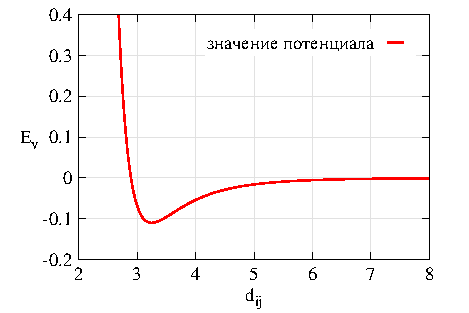
\includegraphics[width=1.0\textwidth]{images/vdwfunc}
	
	\end{columns}
	
\end{frame}



% 4
\begin{frame}{Потенциал Кулона}
	\fontsize{11}{15}\selectfont
	\hangindent=-0.5cm
	\hangafter=-1 \noindent
	\setlength{\leftmargini}{20pt}
	
	\vspace{15pt}
	
	\centering
	\scalebox{1.2}{$\displaystyle E_c = \sum_{i,j}\left(\frac{1}{4 \pi \varepsilon_r} \frac{q_i q_j}{d_{ij}}\left[\frac{d_{ij}^2}{k^2} - \frac{2d_{ij}}{k} + 1\right]\right)$}
	
	
	\begin{columns}[c]
	\column{.5\textwidth}
	
	\vspace{-5pt}

	\begin{itemize}
	\setbeamercolor{itemize item}{fg=myblue!60}
	\setlength\itemsep{1mm}
	\item \scalebox{1.2}{$d_{ij}$} -- евклидово расстояние между \\ центрами атомов
	\item \scalebox{1.2}{$q_i$} и \scalebox{1.2}{$q_j$} -- фиксированные частичные \\ атомные заряды 
	\item \scalebox{1.2}{$\varepsilon_r$} -- диэлектрическая константа	
	\item \scalebox{1.2}{$k$} -- коэффициент отсечения 14 \AA
	\end{itemize}

	\column{.5\textwidth}
	
	\vspace{20pt}
	
	\centering
	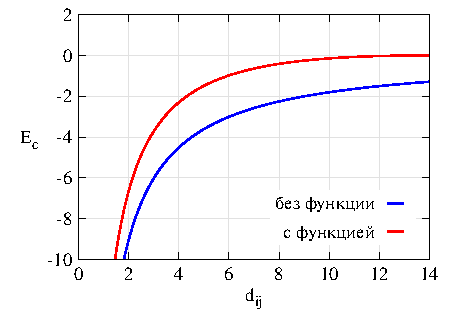
\includegraphics[width=1.0\textwidth]{images/elecfunc}
	
	\end{columns}

\end{frame}



% 5
\begin{frame}{Неявный растворитель}
	\fontsize{11}{15}\selectfont
	\hangindent=-0.5cm
	\hangafter=-1 \noindent
	\setlength{\leftmargini}{20pt}
	
	\vspace{-5pt}
	
	\centering
	\scalebox{1.2}{$\displaystyle E_s = \sum_i \Delta G_i + \sum_{i,j} \left( \frac{1}{2 \pi \sqrt{\pi}} \left[ -\Delta G_i e^{-\left( \tfrac{d_{ij} - {R_i}^{\textquotesingle}}{\lambda_i} \right)^2} - \Delta G_j e^{-\left( \tfrac{d_{ij} - {R_j}^{\textquotesingle}}{\lambda_j} \right)^2} \right] \right)$}
	
	\vspace{+20pt}
	
	\begin{itemize}
	\setbeamercolor{itemize item}{fg=myblue!60}
	\setlength\itemsep{1mm}
	\item \scalebox{1.2}{$d_{ij}$} -- евклидово расстояние между центрами атомов
	\item \scalebox{1.2}{$\lambda_i$} и \scalebox{1.2}{$\lambda_j$} -- размеры гидратных оболочек атомов
	\item \scalebox{1.2}{${R_i}^{\textquotesingle}$} и \scalebox{1.2}{${R_j}^{\textquotesingle}$} -- Ван-Дер-Ваальсовы радиусы атомов, которые соответствуют половине расстояния в потенциале Леннард-Джонса
	\item \scalebox{1.2}{$\Delta G_{i}$} и \scalebox{1.2}{$\Delta G_{j}$} -- энергии гидратации в зависимости от типа атома

	\end{itemize}
	
\end{frame}



% 6
\begin{frame}{Реализация оценочной функции}

	\fontsize{11}{12}\selectfont
	\hangindent=-0.5cm
	\hangafter=-1 \noindent
	\setlength{\leftmargini}{20pt}
	
	\vspace{-5pt}	
	Алгоритм прямого перебора -- $O(n^2{\cdot}k{\cdot}(k-1)/2)$
	
	\begin{itemize}
		\item $k$ -- количество цепей
		\item $n$ -- количество атомов в~одной цепи
	\end{itemize}		
	
	\vspace{4mm}	
	
	Алгоритм с использованием k-d дерева	-- $O(k^2 \cdot n \cdot build)$
	
	\begin{itemize}
		\item $k$ --~количество цепей
		\item $n$ --~количество атомов в~цепи, по которым будет построено k-d-дерево
		\item $build$ -- ~$O(n \cdot \log_{2}{n})$
	\end{itemize}
	
	\vspace{4mm}	
	
	В~общем случае, сложность поиска всех соседей в~k-d-дереве составляет $O(\log_{2}{n} + k)$, где $n$ --~количество точек в~дереве, а~$k$~--~количество найденных соседей в~заданном радиусе сферы взаимодействия атома.

\end{frame}



% 7
\begin{frame}{Результаты оптимизации с использованием k-d дерева}
	\fontsize{11}{12}\selectfont
	\hangindent=-0.5cm
	\hangafter=-1 \noindent
	\setlength{\leftmargini}{20pt}
	
	\centering
	\vspace{-3pt}
	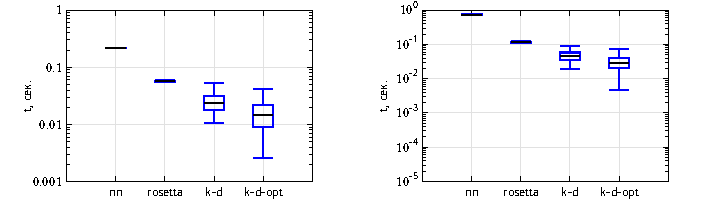
\includegraphics[scale=0.9]{images/bxpt.pdf}
	\vspace{4mm}
	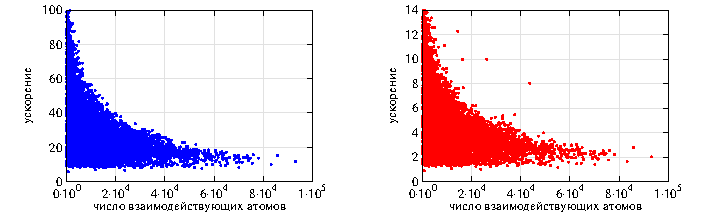
\includegraphics[scale=0.9]{images/accel.pdf}
	
\end{frame}



% 8
\begin{frame}{Верификация выполняемых оценок}
	\fontsize{11}{12}\selectfont
	\hangindent=-0.5cm
	\hangafter=-1 \noindent
	\setlength{\leftmargini}{20pt}
	
	\centering
	\vspace{-3pt}
	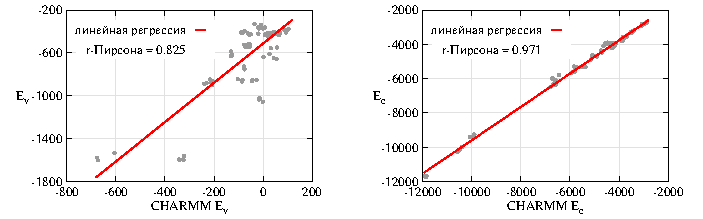
\includegraphics[scale=0.9]{images/first.pdf}
	\vspace{4mm}
	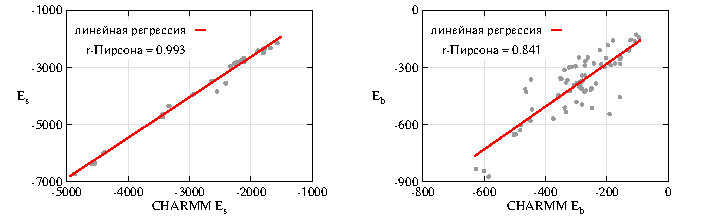
\includegraphics[scale=0.9]{images/second.pdf}
	
\end{frame}



% 9
\begin{frame}{Верификация выполняемых оценок}
	\fontsize{11}{12}\selectfont
	\hangindent=-0.5cm
	\hangafter=-1 \noindent
	\setlength{\leftmargini}{20pt}
	
	\centering
	\vspace{-3pt}
	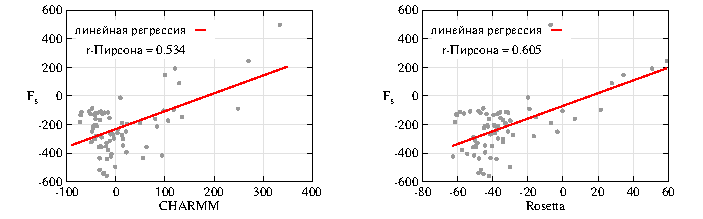
\includegraphics[scale=0.9]{images/third.pdf}
	
	\vspace{4mm}
	\[\text{F}_{\text{s}}=F_{s}^{AB} - \left[F_{s}^{A} + F_{s}^{B}\right]\]
	
	\begin{itemize}
		\item $F_{s}^{AB}$, $F_{s}^{A}$ и $F_{s}^{B}$ найдены с~помощью разработанной оценочной функции значения.
	\end{itemize}
	
\end{frame}



% 10
\begin{frame}{Заключение}
	\fontsize{11}{12}\selectfont
	\hangindent=-0.5cm
	\hangafter=-1 \noindent
	\setlength{\leftmargini}{20pt}
	
	\vspace{-5pt}

Результаты:
\begin{itemize}
	\item Разработана и реализована оценочная функция с~использованием набора параметров силового поля CHARMM в~рамках библиотеки PSM. 
	\item Выполнена оптимизация процедуры поиска взаимодействующих пар атомов с~помощью применения структуры данных k-d-дерево.
	\item Проведены различные численные эксперименты, демонстрирующие приемлемую высокую корреляцию оценок с~результатами силовых полей CHARMM и~Rosetta.
	\item На примере двух белков продемонстрировано преимущество применения структуры данных k-d-дерево для поиска взаимодействующих пар атомов.
	\item Результаты работы представлены на всероссийской конференции~<<Информационно-телекоммуникационные технологии и математическое моделирование высокотехнологичных систем 2023>>, которая проходила 17-21~апреля~2023 в году в~Москве.
\end{itemize}

\end{frame}



% 10
\begin{frame}
	\fontsize{20}{25}\selectfont
	
	
	\begin{columns}[c]
		\column{.5\textwidth}
		\centering
		
		\definecolor{myblue}{RGB}{51, 51, 178}
		\setbeamercolor{block body example}{bg=myblue}
		\begin{exampleblock}{}
			{
				\vskip3mm
				\begin{center}
					\textcolor{white}{Спасибо за внимание!}
				\end{center}
				\vskip5mm
			}
		\end{exampleblock}
		
	\end{columns}
	
\end{frame}


\end{document} 
